\subsection{Scaler}

\subsubsection*{Code}

\inputgroovy[label=RunScaler.groovy]{../ChapterExercises/src/c5/RunScaler.groovy}

\inputgroovy[label=Scale.groovy]{../ChapterExercises/src/c5/Scale.groovy}

\subsubsection*{Results}

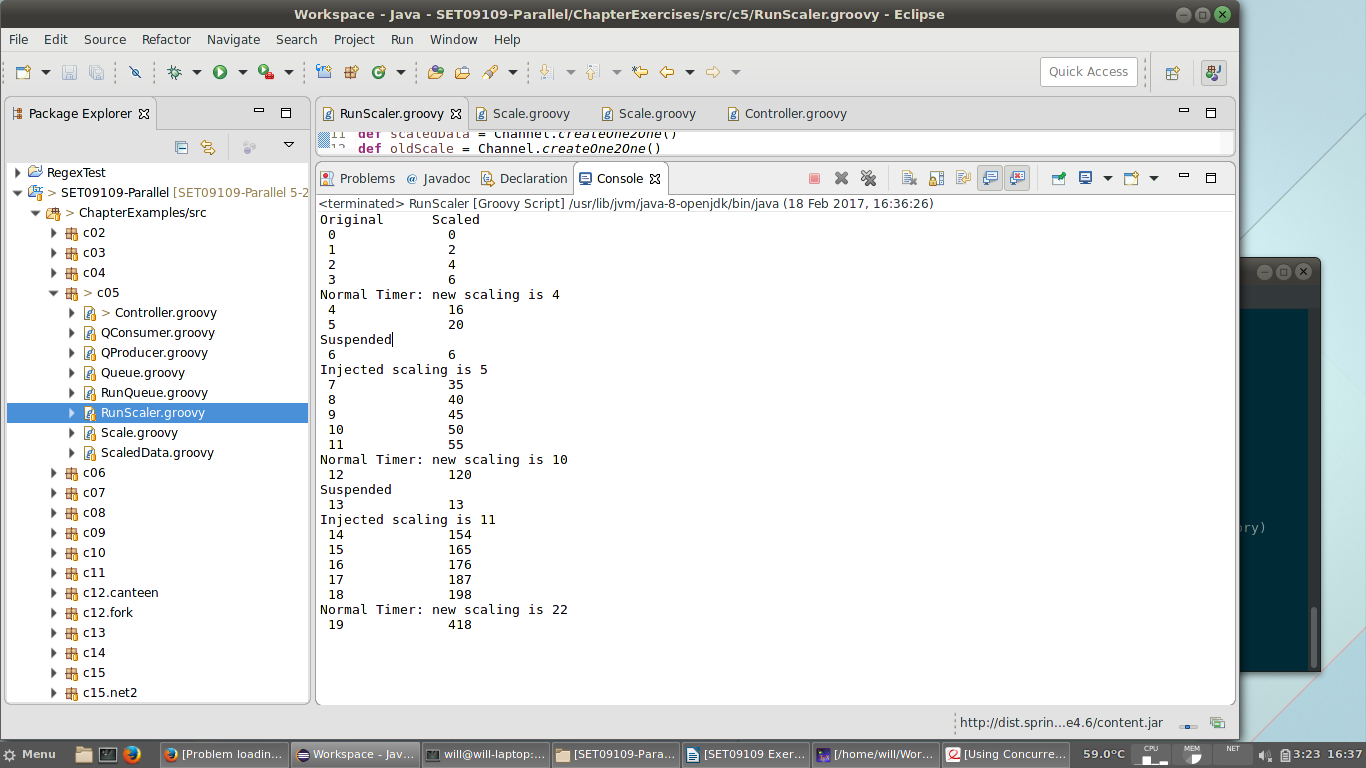
\includegraphics[width=\textwidth]{img/screenshots/5-2.png}

\subsubsection*{Questions}

\paragraph{Which is the more elegant formulation? Why?}

I believe the precondition solution to be more elegant for the following reasons.

\begin{enumerate}
	\item In the nested loop solution there are two different methods for reading from the inChannel.  This breaks the DRY principle.

	\item In the nested loop solution there are two while loops.  This makes it slightly harder to elegantly shut down the process.

	\item The precondition solution allows for easier updating.  If, for example, it was decided that while suspended the timer should still run the nested solution would require another case in the suspended loop.  The precondition solution, however, would only require the \mintinline{groovy}{preCon[TIMER] = false} line to be removed.

\end{enumerate}
